\documentclass{article}
\usepackage{amsmath,amssymb}
\usepackage{float,graphicx}
\usepackage{enumitem}
\usepackage[letterpaper]{geometry}
\usepackage[colorlinks]{hyperref}

\title{Precalculus Practice Problems: Midterm 1}
\author{Alan Zhou}
\date{2024-2025}

\setlength{\parindent}{0pt}
\setlength{\parskip}{3pt plus 1pt minus 1pt}

\renewcommand{\bar}[1]{\overline{#1}}
\renewcommand{\Re}{\operatorname{Re}}
\renewcommand{\Im}{\operatorname{Im}}

\DeclareMathOperator{\chd}{chd}


\begin{document}

\maketitle

%The focus of these review problems is on the material covered in Weeks 25 through 35, but keep in mind that prior material can still appear on the exam.

\tableofcontents

\section{Trig (I): Right Triangle and Unit Circle}

\subsection{Review problems}

\begin{enumerate}
\item \emph{Unit conversions for angles.}
\begin{enumerate}
\item 360 degrees to radians
\item $\pi$ radians to degrees
\item 60 degrees to radians
\item $3\pi/4$ radians to degrees
\item $\pi/5$ degrees to radians
\end{enumerate}
\item \emph{Trig functions as ratios of lengths.} Let $ABC$ be a triangle with a right angle at $B$. Suppose $AB = 8$ and $BC = 15$.
\begin{enumerate}
\item Evaluate $\tan A$ and $\cot A$.
\item Find the length of $AC$.
\item Evaluate $\sin A$, $\cos A$, $\sec A$, and $\csc A$.
\end{enumerate}
\item \emph{Using one trig function to compute another.} Throughout, assume $\theta$ is acute.
\begin{enumerate}
\item If $\sin\theta = 1/3$, what is $\cos\theta$?
\item If $\sec\theta = \sqrt{10}$, what is $\tan\theta$?
\item If $\tan\theta = 2/5$, what is $\csc\theta$?
\end{enumerate}
\item \emph{Important acute angles.} Fill in the table below.
\begin{center}
\begin{tabular}{c|c||c|c|c|c|c|c}
$\theta$ (deg) & $\theta$ (rad) & $\sin\theta$ & $\cos\theta$ & $\tan\theta$ & $\sec\theta$ & $\csc\theta$ & $\cot\theta$ \\ \hline
 & & & & & & & \\
30 & & & & & & & \\
 & & & & & & & \\ \hline
 & & & & & & & \\
45 & & & & & & & \\
 & & & & & & & \\ \hline
 & & & & & & & \\
 & $\pi/3$ & & & & & & \\
 & & & & & & & 
\end{tabular}
\end{center}\newpage
\item \emph{Unit circle calculations.} Compute the following.
\begin{enumerate}
\item $\cos(0)$
\item $\sin(150^{\circ})$
\item $\cos(-3\pi/4)$
\item $\sin(7\pi/3)$
\item $\cos(330^{\circ})$
\item $\sin(-\pi/4)$
\end{enumerate}
\item \emph{Unit circle identities.} Express each of the following in terms of $\sin\theta$ and/or $\cos\theta$.
\begin{enumerate}
\item $\sin(\pi - \theta)$
\item $\cos(\pi - \theta)$
\item $\sin(\pi + \theta)$
\item $\cos(\pi + \theta)$
\item $\sin(-\theta)$
\item $\cos(-\theta)$
\item $\sin(\frac{\pi}{2} - \theta)$
\item $\cos(\frac{\pi}{2} - \theta)$
\item $\sin(\frac{\pi}{2} + \theta)$
\item $\cos(\frac{\pi}{2} + \theta)$
\end{enumerate}
\item \emph{Some triangle geometry.} In acute triangle $ABC$, it is given that $AB = 13$, that $BC = 14$, and that $\sin B = 12/13$.
\begin{enumerate}
\item Find the area of triangle $ABC$.
\item Find the length of $AC$.
\item Find $\sin A$.
\end{enumerate}
\end{enumerate}


\subsection{Challenge problems}

\begin{enumerate}\setcounter{enumi}{7}
\item % chord
\item % parallax
\item % unit circle pythagorean triples 
\end{enumerate}


%\subsection{Answers}
\section{Trig (II): Graphs and Inverses}

\subsection{Review problems}

\begin{enumerate}
\item \emph{The six basic graphs.} Match each of the graphs below to one of the six basic trig functions.
\begin{figure}[H]
\centering
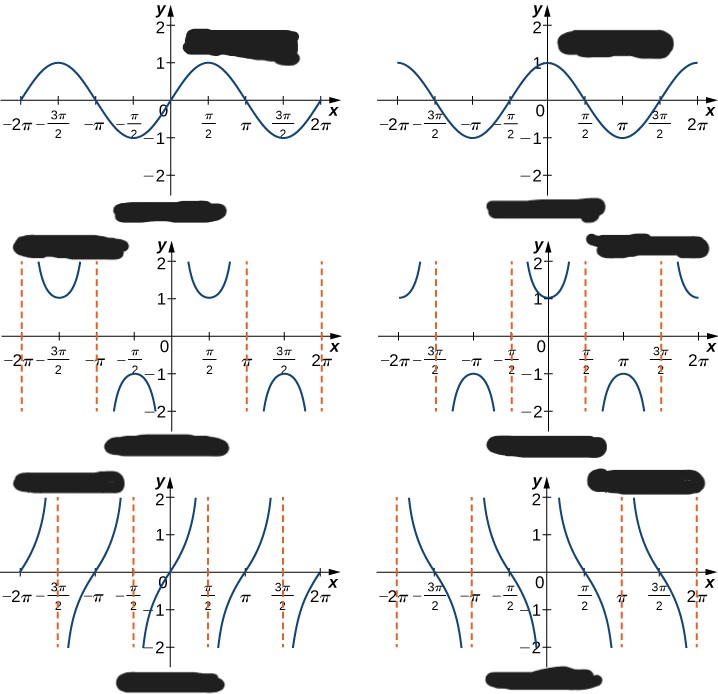
\includegraphics[scale=0.7]{img-trig-graphs.jpg}
\end{figure}
\item \emph{Period and frequency.} A function $f:\mathbb{R}\to\mathbb{R}$ is \emph{periodic} if there is a non-zero real number $T$ such that $f(x + T) = f(x)$ for all real $x$. Any such $T$ is a \emph{period} of $f$, and the smallest such positive $T$, if it exists, is the \emph{fundamental period} of $f$. If $f$ is a periodic function with fundamental period $T$, the \emph{natural frequency} of $f$ is $\nu = 1/T$ while the \emph{angular frequency} of $f$ is $\omega = 2\pi/T = 2\pi\nu$. Usually, ``the period'' of a periodic function means its fundamental period, while ``a period'' can be any period (not just the fundamental period). For each of the six basic trig functions, what are the period, natural frequency, and angular frequency?
\item \emph{Transformed sinusoidal waves.} For each of the following functions $\mathbb{R}\to\mathbb{R}$, find the period, amplitude, and phase shift relative to $\sin(\omega x)$, where $\omega$ is the angular frequency of the function.
\begin{enumerate}
\item $\sin x$
\item $\cos x$
\item $3\sin(5x - \tfrac{\pi}{7})$
\item $2\sin(2x) - 2\cos(2x)$
\end{enumerate}
\item \emph{Domain and range.} What are the standard domains and ranges of $\arcsin$, $\arccos$, and $\arctan$?\newpage
\item \emph{Calculating inverses.}
\begin{enumerate}
\item $\arcsin(1/2)$
\item $\arccos\left(-1/\sqrt{2}\right)$
\item $\arcsin\left(-\sqrt{3}/2\right)$
\item $\arctan(-1)$
\item $\arcsin(\sin(7\pi/6))$
\item $\cos(\arccos(-1/3))$
\item $\cos(\arctan(1/2))$
\end{enumerate}
\item \emph{Counting solutions.} Find the number of solutions for $x$ in each of the following equations.
\begin{enumerate}
\item $\sin\theta = 0.5$ when $0\leq\theta < 2\pi$
\item $\cos\theta = -2$ when $0\leq\theta < 2\pi$
\item $\sec\theta = 1$ when $-\pi < \theta\leq\pi$
\item $\tan\theta = 1$ when $-\pi < \theta\leq\pi$
\item $\sin(3\theta) = 0.2024$ when $0\leq\theta < 10\pi$
\item $\cos(\frac{22}{7}\theta) = 0.5$ when $-20 < \theta < 20$
\end{enumerate}
\item What are the standard domains and ranges of $\sec^{-1}$, $\csc^{-1}$, and $\cot^{-1}$?
\end{enumerate}


\subsection{Challenge problems}

\begin{enumerate}\setcounter{enumi}{7}
\item Karen has a calculator which only has seven buttons: $\sin$, $\cos$, $\tan$, $\arcsin$, $\arccos$, $\arctan$, and Reset. The first six apply these functions to the number in the display, while Reset changes the display back to its default state of showing 0. All calculations assume radian measure.
\begin{enumerate}
\item Starting from a positive real number $x$ in the display, show that there is a sequence of buttons that changes the display to $1/x$.
\item Starting from a non-negative real number $x$ in the display, show that there is a sequence of buttons that changes the display to $\sqrt{x^2 + 1}$.
\item Show that for every positive rational number $q$, there is a sequence of buttons that changes the display from $0$ to $\sqrt{q}$.
\end{enumerate}
\item Find the period of the following functions, or show that no period exists.
\begin{enumerate}
\item $\sin(3x) + \sin(4x)$
\item $\sin(20x) + \sin(24x)$
\item $\sin(x) + \sin(\sqrt{2}x)$
\end{enumerate}
\item A function $f:\mathbb{C}\to\mathbb{C}$ is \emph{doubly-periodic} if there are non-zero constants $u,v\in\mathbb{C}$ such that $u/v$ is non-real and $f(z) = f(z + u) = f(z + v)$ for all complex numbers $z$. Write down an example of a non-constant doubly-periodic function.
\end{enumerate}


\newpage
\subsection{Answers}

\begin{enumerate}
\item top left is sine; top right is cosine;\par
middle left is cosecant; middle right is secant;\par
bottom left is tangent; bottom right is cotangent
\item sine, cosine, secant, cosecant have period $2\pi$, natural frequency $\frac{1}{2\pi}$, angular frequency 1;\par 
theirangent, cotangent have period $\pi$, natural frequency $\frac{1}{\pi}$, angular frequency 2
\item \begin{enumerate}
\item period $2\pi$; amplitude $1$; phase shift $0$
\item period $2\pi$; amplitude $1$; phase shift $-\pi/2$ since $\cos x = \sin\left(x + \frac{\pi}{2}\right)$
\item period $2\pi/5$; amplitude $3$; phase shift $\pi/35$
\item period $\pi$; amplitude $2\sqrt{2}$ since $2\sin(2x) - 2\cos(2x) = 2\sqrt{2}\sin\left(2x - \frac{\pi}{4}\right)$; phase shift $\pi/8$
\end{enumerate}
\item arcsin has domain $[-1,1]$ and range $[-\pi/2, \pi/2]$;\par
arccos has domain $[-1,1]$ and range $[0,\pi]$;\par
arctan has domain $\mathbb{R}$ and range $(-\pi/2, \pi/2)$
\item \begin{enumerate}
\item $\pi/6$
\item $3\pi/4$
\item $-\pi/3$
\item $-\pi/4$
\item $-\pi/6$
\item $-1/3$
\item $2/\sqrt{5}$
\end{enumerate}
\item \begin{enumerate}
\item 2
\item 0
\item 1
\item 2
\item 30
\item 40
\end{enumerate}
\item $\sec^{-1}$ has domain $(-\infty,-1]\cup [1,+\infty)$ and range $[0,\pi/2)\cup (\pi/2,\pi]$;\par 
$\csc^{-1}$ has domain $(-\infty,-1]\cup [1,+\infty)$ and range $[-\pi/2,0)\cup (0,\pi/2]$;\par
$\cot^{-1}$ has domain $\mathbb{R}$ and range $(0,\pi)$
\item First note for any acute angle $\theta$ that $C(\theta) = \arccos(\sin\theta) = \pi/2 - \theta$.
\begin{enumerate}
\item Given $x > 0$, the angle $\arctan x$ is acute, so $A(x) = \tan(C(\arctan x)) = 1/x$.
\item Given $x\geq 0$, we have $\cos(\arctan x) = 1/\sqrt{x^2 + 1}$, so $B(x) = A(\cos(\arctan x)) = \sqrt{x^2 + 1}$.
\item Let $q = m/n$ where $\gcd(m,n) = 1$. Note that $B^{-1}(\sqrt{q}) = \sqrt{q - 1}$ and $A^{-1}(\sqrt{q}) = \sqrt{1/q}$ correspond to steps of the Euclidean algorithm on $m$ and $n$. Since $\gcd(m,n) = 1$, we can work backwards until we reach $0/1 = 0$. Running our steps in reverse gives us a sequence of button presses that goes from $0$ to $\sqrt{q}$.
\end{enumerate}
\item For each part, denote the function by $f$ and the period by $T$.
\begin{enumerate}
\item From $f(T) = f(0)$, we get $\sin(3T) + \sin(4T) = 0$, while from $f(\pi) = f(\pi + T)$, we get $-\sin(3T) + \sin(4T) = 0$, which means $\sin(3T) = \sin(4T) = 0$. The only values which satisfy this are multiples of $\pi$. However, $f(-\pi/2) = 1$ while $f(\pi/2) = -1$, so $T\neq\pi$. Therefore, the smallest positive real number that $T$ could be is $2\pi$, and $f(x + 2\pi) = f(x)$ for all $x$ since each term individually has period $2\pi$, so $T = 2\pi$ works.
\item From $f(T) = f(0)$, we get $\sin(20T) + \sin(24T) = 0$, while from $f(\pi/4) = f(\pi/4 + T)$, we get $-\sin(20T) + \sin(24T) = 0$, so $\sin(20T) = \sin(24T) = 0$. This holds when $T$ is a multiple of $\pi/4$, and by similar reasoning to part (a), $\pi/4$ fails while $T = \pi/2$ works.
\item From $f(T) = f(0)$, we get $\sin T + \sin(\sqrt{2}T) = 0$. However, from $f(2\pi) = f(2\pi + T)$,
\begin{equation*}
\sin(2\sqrt{2}\pi) = \sin T + \sin(2\sqrt{2}\pi + \sqrt{2}T).
\end{equation*}
Subtracting these two equations and rearranging,
\begin{equation*}
\sin(2\sqrt{2}\pi + \sqrt{2}T) = \sin(2\sqrt{2}\pi) + \sin(\sqrt{2}T).
\end{equation*}
In general,
\begin{equation*}
\sin a + \sin b = \sin(a + b) = \sin a\cos b + \sin b\cos a
\end{equation*}
only when $\sin b = 0$ and $\cos b = 1$ or when $\sin b = -\sin a$ and $\cos b = \cos a$; this can be proved by holding $a$ fixed and solving for $\sin b$ and $\cos b$ using $\sin^2 b + \cos^2 b = 1$. With $a = 2\sqrt{2}\pi$ and $b = \sqrt{2}T$, the first case would give us $\sin T = \sin(\sqrt{2}T) = 0$. However, this would force both $T$ and $\sqrt{2}T$ to be multiples of $\pi$, which is impossible when $T$ is non-zero since $\sqrt{2}$ is irrational. For the second case, the conditions on $\sin b$ and $\cos b$ tell us that $a + b = 2m\pi$ for an integer $m$. We can run the exact same argument with $f(-2\pi) = f(-2\pi + T)$ to show that $a' + b = 2n\pi$ for an integer $n$, where $a' = -2\sqrt{2}\pi$. Subtracting gives us $4\sqrt{2}\pi = (2m - 2n)\pi$, which is impossible by irrationality of $\sqrt{2}$. Hence $f$ has no period.
\end{enumerate}
\item Given two periodic functions $g,h:\mathbb{R}\to\mathbb{R}$, we can define $f:\mathbb{C}\to\mathbb{C}$ by $f(x + yi) = g(x)h(y)$ for $x,y$ real, and this will be doubly-periodic. In complex notation, this is
\begin{equation*}
f(z) = g\left(\frac{z + \bar{z}}{2}\right)h\left(\frac{z - \bar{z}}{2i}\right).
\end{equation*}
Writing down an example that only uses $z$ (without $\bar{z}$ or $\lvert z\rvert$) turns out to be substantially more difficult. A classic example central to the theory of ``nice'' doubly-periodic functions is the \emph{Weierstrass elliptic function}: if we want the periods to take the form $m\omega_1 + n\omega_2$, where $\omega_1/\omega_2$ is non-real and $m,n$ are integers, then we define
\begin{equation*}
\wp(z) = \sum_{m = -\infty}^{\infty}\sum_{n = -\infty}^{\infty} f_{m,n}(z),\quad f_{m,n}(z) = \begin{cases} \frac{1}{[z - (m\omega_1 + n\omega_2)]^2} - \frac{1}{(m\omega_1 + n\omega_2)^2} & (m,n)\neq (0,0); \\ \frac{1}{z^2} & (m,n) = (0,0). \end{cases}
\end{equation*}
\end{enumerate}
%\section{Special Functions}

\subsection{Review problems}

\begin{enumerate}
\item Let $f(x) = 4x^3 - 6x^4 + 2x - 1$ and $g(x) = 3x^4 + x^2 + 9$ and $h(x) = \sqrt{x^2 + 1}$.
\begin{enumerate}
\item Which of $f$, $g$, and $h$ are polynomial functions?
\item Evaluate $f(0)$ and $g(1)$.
\item Simplify $f(x) + g(x)$ and $f(x)\cdot g(x)$.
\item Compute $\deg f(x)$ and $\deg g(x)$.
\item Is there a constant $a$ for which $f(x) + a\cdot g(x)$ has degree less than $4$? If so, what is the value of $a$ and the degree of $f(x) + a\cdot g(x)$ for that value? If not, explain why not.
\end{enumerate}
\item Let $p(x) = x^4 + 9x^3 + 28x^2 + 39x + 21$. This polynomial has no integer roots, but there are positive integers $a,b,c,d$ such that 
\begin{equation*}
p(x) = (x^2 + ax + b)(x^2 + cx + d).
\end{equation*}
Find all \underline{real} roots of $p(x)$.
\item Solve each of the following equations for $x$.
\begin{enumerate}
\item $\sqrt[6]{625} = 5^x$
\item $9^{1 + x} = 27^{1 + 1/x}$
\item $4^x - 2^x = 56$
\end{enumerate}
\item (Calculator allowed) Janelle puts \$10,000 into an account that earns $4\%$ interest compounded annually. How much money will there be in the account after $18$ years?
\item Compute each of the following logarithms without a calculator (some are undefined).
\begin{enumerate}
\item $\log_7(49)$
\item $\log_2(64)$
\item $\log_{27}(9)$
\item $\log_5(1)$
\item $\log_4(0)$
\item $\log_6(-6)$
\item $\log_8(1/4)$
\item $\log_{12}\left(2\sqrt[3]{18}\right)$
\end{enumerate}
\item Find the domain and range of the function $f(x) = \log_{10}\left(\sqrt{100 - x^2}\right)$.
\item Find the values of $a$, $b$, and $c$ which make the following function continuous:
\begin{equation*}
f(x) = \begin{cases} x^2 - 3 & x\leq -1; \\ ax + b & -1 < x\leq 2; \\ \frac{2x^2 - 3x - 9}{x^2 - 4x + 3} & x > 2\text{ and }x\neq 3; \\ c & x = 3. \end{cases}
\end{equation*}
\end{enumerate}


\subsection{Challenge problems}

\begin{enumerate}[resume]
\item Let $p(x) = (1 + x)^{20}$.
\begin{enumerate}
\item Find the sum of the coefficients of $p(x)$.
\item Find the sum of the coefficients of $p(x - 1)$.
\item (Very challenging) Find the sum of the coefficients of the terms of $p(x)$ whose degrees are multiples of $4$.
\end{enumerate}
\item (Calculator allowed)
\begin{enumerate}
\item Let $E(i,m)$ denote the \emph{effective annual interest rate} for a nominal annual interest rate $i$ compounded $m$ times per year. That is, for any whole number of years, compounding annually at a rate of $E(i,m)$ results in the same balance as compounding $m$ times per year with a nominal annual interest rate $i$.\par Write down a formula for $E(i,m)$ in terms of $i$ and $m$, then compute $E(4\%, 12)$.
\item Let $F(i,m)$ be the solution to the equation $E(F(i,m),m) = i$. Compute $F(4\%, 12)$.
\item If we hold $i$ fixed, then as $m$ gets larger and larger, $F(i,m)$ approaches a value called the \emph{force of interest}. For the interest rate $i = 4\%$, compute the force of interest to three decimal places.
\end{enumerate}
\item Compute $(\log_4 5)(\log_5 6)(\log_6 7)(\log_7 8)$ without a calculator.
\end{enumerate}


\newpage
\subsection{Answers}

\begin{enumerate}
\item \begin{enumerate}
\item $f$ and $g$ are polynomials, $h$ is not 
\item $f(0) = -1$ and $g(1) = 13$
\item \begin{align*}
f(x) + g(x) &= -3x^4 + 4x^3 + x^2 + 2x + 8 \\
f(x)\cdot g(x) &= -18x^8 + 12x^7 - 6x^6 + 10x^5 - 57x^4 + 38x^3 - x^2 + 18x - 9
\end{align*}
\item $\deg f(x) = \deg g(x) = 4$
\item When $a = 2$,
\begin{equation*}
f(x) + a\cdot g(x) = 4x^3 + 2x^2 + 2x + 17
\end{equation*}
so $\deg (f(x) + a\cdot g(x)) = 3$.
\end{enumerate}
\item We can suppose that $b\leq d$, as otherwise we simply swap the two factors of $p(x)$. Expanding,
\begin{align*}
a + c &= 9, \\
b + ac + d &= 28, \\
ad + bc &= 39, \\
bd &= 21.
\end{align*}
Since $a,b,c,d$ are positive integers, either $b = 1$ and $d = 21$ or $b = 3$ and $d = 7$. In the first case, we have $a + c = 9$ and $21a + b = 39$, but this is not satisfied by positive integers. Thus we are in the second case, so $a + c = 9$ and $7a + 3b = 39$. This system has solution $a = 3$ and $c = 6$, and we can check the other equations (or by expanding from scratch) to see that
\begin{equation*}
p(x) = (x^2 + 3x + 3)(x^2 + 6x + 7).
\end{equation*}
If $r$ is a root of $p(x)$, then $p(r) = 0$, so either $r^2 + 3r + 3 = 0$ or $r^2 + 6r + 7 = 0$. By the quadratic formula, the first case gives us
\begin{equation*}
r = \frac{-3\pm\sqrt{-3}}{2},
\end{equation*}
which are non-real roots, while the second case gives us
\begin{equation*}
r = \frac{-6\pm\sqrt{8}}{2} = \boxed{-3\pm\sqrt{2}}.
\end{equation*}
\item 
\end{enumerate}
%\section{Sequences and Series}

\subsection{Review problems}

\begin{enumerate}
\item Identify, for each of the following sequences, whether they could be arithmetic, geometric, both, or neither. For any arithmetic sequence, identify the common difference. For any geometric sequence, identify the common ratio. 
\begin{enumerate}
\item $1, 1, 1, 1, 1, \ldots$
\item $2, -2, 2, -2, 2, \ldots$
\item $1, 1, 2, 3, 5, \ldots$
\item $5, 11, 17, 23, 29, \ldots$
\item $\frac{1}{\sqrt{2}}, \sqrt{2}, \frac{3}{2}\sqrt{2}, \sqrt{8}, \frac{5\sqrt{2}}{2}, \ldots$
\end{enumerate}
\item Compute the arithmetic series
\begin{equation*}
3 + 5 + 7 + 9 + \cdots + 89.
\end{equation*}
\item The sum of the first $6$ terms of an arithmetic sequence is $114$, and the sum of the next $5$ terms is $-15$. What is the least positive integer $N$ for which the sum of the first $N$ terms of the series is (strictly) negative?
\item (Calculator permitted) Jo puts $\$1000$ into a savings account at the beginning of every year starting at the beginning of 2024. The account earns $2\%$ nominal annual interest, compounded quarterly. How much money will there be in her account at the end of 2050?
\item When
\begin{equation*}
0.304\,878\,048\,780\,487\,804\,878\,\ldots = 0.3\overline{04878}
\end{equation*}
is expressed as a fraction in lowest terms, the numerator is $25$. What is the denominator?
\item \begin{enumerate}
\item Find constants $A$ and $B$ such that
\begin{equation*}
\frac{1}{n(n + 2)} = \frac{A}{n} + \frac{B}{n + 2}
\end{equation*}
for all positive integers $n$.
\item Evaluate the series
\begin{equation*}
\frac{1}{3} + \frac{1}{8} + \frac{1}{15} + \frac{1}{24} + \frac{1}{35} + \frac{1}{48} + \cdots + \frac{1}{9800}.
\end{equation*}
\end{enumerate}
\item For each positive integer $n$, we define $n!$ (read as: ``$n$ factorial'') to be the product of the first $n$ positive integers. The first few factorials are
\begin{equation*}
1! = 1,\quad 2! = 2\cdot 1 = 2,\quad 3! = 3\cdot 2\cdot 1 = 6,\quad 4! = 4\cdot 3\cdot 2\cdot 1 = 24.
\end{equation*}
\begin{enumerate}
\item For which positive integers $n$ is it true that $n! > 2^n$?
\item When the infinite series
\begin{equation*}
\frac{10}{1!} + \frac{10}{2!} + \frac{10}{3!} + \frac{10}{4!} + \frac{10}{5!} + \frac{10}{6!} + \cdots
\end{equation*}
is computed, between what two consecutive positive integers does the value lie?
\end{enumerate}
\end{enumerate}


\subsection{Challenge problems}

\begin{enumerate}[resume]
\item Let $0 < x < 1$ be a real number.
\begin{enumerate}
\item Evaluate the infinite series
\begin{equation*}
1 - x + x^2 - x^3 + x^4 - x^5 + x^6 - x^7 + \cdots \tag{$\dagger$}
\end{equation*}
in terms of $x$.
\item As $x$ gets closer and closer to $1$, what value does the infinite series $(\dagger)$ approach?
\item When we compute the sum of the first $n$ terms of
\begin{equation*}
1 - 1 + 1 - 1 + 1 - 1 + 1 - 1 + \cdots
\end{equation*}
for larger and larger values of $n$, do these sums approach your answer to part (b)?
\end{enumerate}
\item For each positive integer $n$, let $A_n$ be the sum of the first $n$ squares and let $T_n$ be the sum of the first $n$ positive integers.
\begin{enumerate}
\item Show that $T_n = \frac{n(n + 1)}{2}$.
\item Show that for each positive integer $n$,
\begin{equation*}
(n + 1)^3 - 1 = 3A_n + 3T_n + n.
\end{equation*}
\emph{Hint: Expand $(k + 1)^3 - k^3$.}
\item Evaluate $A_{100}$.
\end{enumerate}
\item (Basel problem and related sums) It was found by Leonhard Euler in 1734 that
\begin{equation*}
\frac{1}{1^2} + \frac{1}{2^2} + \frac{1}{3^2} + \frac{1}{4^2} + \frac{1}{5^2} + \cdots = \frac{\pi^2}{6}.
\end{equation*}
\begin{enumerate}
\item Compute
\begin{equation*}
\frac{1}{2^2} + \frac{1}{4^2} + \frac{1}{6^2} + \frac{1}{8^2} + \frac{1}{10^2} + \cdots.
\end{equation*}
\item Compute
\begin{equation*}
\frac{1}{1^2} + \frac{1}{3^2} + \frac{1}{5^2} + \frac{1}{7^2} + \frac{1}{9^2} + \cdots.
\end{equation*}
\end{enumerate}
\end{enumerate}


\newpage
\subsection{Answers}

\begin{enumerate}
\item \begin{enumerate}
\item Arithmetic (common difference 0) and geometric (common difference 1)
\item Geometric with common ratio $-1$
\item Neither arithmetic nor geometric
\item Arithmetic with common difference 6
\item Arithmetic with common difference $\sqrt{2}/2$
\end{enumerate}
\item Let $n$ be the number of terms in the series. The common difference is 2, so since there are $n - 1$ ``steps'' from the first term to the last term,
\begin{equation*}
3 + 2(n - 1) = 89\implies n = 44.
\end{equation*}
Using the formula from class, the value of the series is 
\begin{equation*}
\frac{1}{2}\cdot 44\cdot (3 + 89) = \boxed{2024}.
\end{equation*}
\item Let $a$ be the first term and $d$ be the common difference. Denoting the $n$-th term of the sequence by $a_n$, the relevant terms for the two given series are
\begin{align*}
a_1 &= a, & a_6 &= a + 5d; \\
a_7 &= a + 6d, & a_{11} &= a + 10d.
\end{align*}
The sum of the first $6$ terms gives us the equation
\begin{equation*}
114 = \frac{1}{2}\cdot 6\cdot (a_1 + a_6) = 6a + 15d,
\end{equation*}
while the sum of the next $5$ terms gives us the equation 
\begin{equation*}
-15 = \frac{1}{2}\cdot 5\cdot (a_7 + a_{11}) = 5a + 40d.
\end{equation*}
Solving this system, we get $a = 29$ and $d = -3$.\par 
From here, we want to find the least $N$ for which the sum of the first $N$ terms,
\begin{equation*}
\frac{1}{2}\cdot N\cdot (29 + [29 - 3(N - 1)]),
\end{equation*}
is negative. Simplifying, we have the inequality
\begin{equation*}
\frac{N}{2}(61 - 3N) < 0,
\end{equation*}
which is first satisfied when $N = \boxed{21}$.
\item After a year passes, the amount of money in the account is multiplied by
\begin{equation*}
r = \left(1 + \frac{0.02}{4}\right)^4 = 1.005^4.
\end{equation*}
The first $\$1000$ is multiplied by $r^{27}$, since its contribution to the account is present for $27$ years (the \emph{beginning} of 2024 to the \emph{end} of 2050). The next $\$1000$ is multiplied by $r^{26}$, then the next $\$1000$ is multiplied by $r^{25}$, and so on. We stop at the last deposit of $\$1000$, which is multiplied by $r^1$. The total in the account by the end of 2050 is then 
\begin{align*} 
\$1000\cdot r^{27} + \$1000\cdot r^{26} + \cdots + \$1000\cdot r^1 &= \$1000\cdot (r^1 + r^2 + \cdots + r^{27}) \\
&= \$1000\cdot\frac{r^{28} - r^1}{r - 1} \\
&\approx \$36\,132.
\end{align*} 
\item First, the infinite geometric series formula gives us 
\begin{align*}
0.\overline{04878} &= \frac{4878}{10^5} + \frac{4878}{10^{10}} + \frac{4878}{10^{15}} + \cdots = \frac{4878}{10^5}\cdot\frac{1}{1 - \tfrac{1}{10^5}} \\
&= \frac{4878}{10^5 - 1} = \frac{4878}{99999} = \frac{542}{11111}.
\end{align*}
(If you are familiar with the Euclidean algorithm, then instead of what follows, it is recommended to use it to find the greatest common divisor and simplify the fraction further that way.) This means that
\begin{align*}
 0.3\overline{04878} &= 0.3 + 0.0\overline{04878} = \frac{3}{10} + \frac{1}{10}\cdot\frac{542}{11111} \\
 &= \frac{33333 + 542}{111110} = \frac{33875}{111110}.
\end{align*}
The problem tells us that when this fraction is fully simplified, the numerator is $25$. This means the greatest common divisor of the numerator and denominator is $33875/25 = 1355$, and the denominator is
\begin{equation*}
\frac{111110}{1355} = \frac{22222}{271} = \boxed{82}.
\end{equation*}
\item \begin{enumerate}
\item Clearing denominators by multiplying both sides by $n(n + 2)$, we need
\begin{equation*}
1 = A(n + 2) + Bn = (A + B)n + 2A
\end{equation*}
for all $n$. This means $2A = 1$, so $A = 1/2$, and $A + B = 0$, so $B = -1/2$.
\item The $n$-th term of the series is $\tfrac{1}{n(n + 2)}$, so 
\begin{align*} 
\frac{1}{3} + \frac{1}{8} + \cdots + \frac{1}{9800} &= \frac{1}{2}\left[\left(\frac{1}{1} - \frac{1}{3}\right) + \left(\frac{1}{2} - \frac{1}{4}\right) + \cdots + \left(\frac{1}{98} - \frac{1}{100}\right)\right] \\
&= \frac{1}{2}\left[\frac{1}{1} + \frac{1}{2} - \frac{1}{99} - \frac{1}{100}\right] \\
&= \frac{1}{2}\cdot\frac{9900 + 4950 - 100 - 99}{9900} = \frac{14651}{19800}.
\end{align*} 
\end{enumerate}
\end{enumerate}


\end{document}
